\documentclass{beamer}

%
% Choose how your presentation looks.
%
% For more themes, color themes and font themes, see:
% http://deic.uab.es/~iblanes/beamer_gallery/index_by_theme.html
%
\mode<presentation>
{
  \usetheme{Madrid}      % or try Darmstadt, Madrid, Warsaw, ...
  \usecolortheme{beaver} % or try albatross, beaver, crane, ...
  \usefonttheme{serif}  % or try serif, structurebold, ...
  \setbeamertemplate{navigation symbols}{}
  \setbeamertemplate{caption}[numbered]
} 

% packages
\usepackage[english]{babel}
\usepackage[utf8]{inputenc}
\usepackage[T1]{fontenc}
\usepackage{graphicx}
\usepackage{wrapfig}
\usepackage{amsmath, amssymb}


%tikz
\usepackage{tikz}
\usetikzlibrary{shapes,snakes,arrows, chains, positioning, shapes.geometric, shapes.symbols,calc,shadows}
\usepackage{tikz-3dplot}
\tdplotsetmaincoords{70}{110}
\usepackage{tikz-cd}
\def\centerarc[#1](#2)(#3:#4:#5)% Syntax: [draw options] (center) (initial angle:final angle:radius)
{ \draw[#1] ($(#2)+({#5*cos(#3)},{#5*sin(#3)})$) arc (#3:#4:#5); }

% commands
\newcommand{\C}{\mathbb{C}}
\newcommand{\Q}{\mathbb{Q}}
\newcommand{\R}{\mathbb{R}}
\newcommand{\Z}{\mathbb{Z}}
\renewcommand{\P}{\mathbb{P}}
\newcommand{\CP}{\mathbb{CP}}

\newcommand{\mA}{\mathcal{A}}
\newcommand{\mB}{\mathcal{B}}
\newcommand{\mC}{\mathcal{C}}
\newcommand{\mE}{\mathcal{E}}
\newcommand{\mF}{\mathcal{F}}
\newcommand{\mG}{\mathcal{G}}
\newcommand{\mK}{\mathcal{K}}
\newcommand{\mO}{\mathcal{O}}
\newcommand{\mH}{\mathcal{H}}
\newcommand{\mI}{\mathcal{I}}
\newcommand{\mT}{\mathcal{T}}
\newcommand{\mL}{\mathcal{L}}
\newcommand{\mN}{\mathcal{N}}
\newcommand{\mP}{\mathcal{P}}
\newcommand{\mQ}{\mathcal{Q}}
\newcommand{\mS}{\mathcal{S}}
\newcommand{\mU}{\mathcal{U}}
\newcommand{\mV}{\mathcal{V}}

\newcommand{\ba}{\mathbf{a}}
\newcommand{\bb}{\mathbf{b}}
\newcommand{\be}{\mathbf{e}}
\newcommand{\bF}{\mathbf{F}}
\newcommand{\bx}{\mathbf{x}}

\newcommand{\mLi}{\mathcal{L}_{\textup{irr}}}
\newcommand{\mLr}{\mathcal{L}_{\textup{red}}}
\newcommand{\p}{\partial}
\newcommand{\iprod}{\mathbin{\lrcorner} \,}

\newcommand{\tL}{\widetilde{L}}
\newcommand{\tM}{\widetilde{M}}
\newcommand{\tH}{\widetilde{H}}
\newcommand{\tmH}{\widetilde{\mH}}
\newcommand{\tx}{\widetilde{x}}
\newcommand{\tp}{\widetilde{p}}
\newcommand{\tX}{\widetilde{X}}
\newcommand{\tD}{\widetilde{D}}
\newcommand{\tY}{\widetilde{Y}}
\newcommand{\tN}{\widetilde{N}}
\newcommand{\tP}{\widetilde{P}}
\newcommand{\tQ}{\widetilde{Q}}
\newcommand{\tV}{\widetilde{V}}
\newcommand{\newpar}{\vspace{0.15in}}

\newcommand{\tv}{\tilde{v}}

\newcommand{\txA}{\textup{A}}
\newcommand{\txB}{\textup{B}}
\newcommand{\txC}{\textup{C}}

\newcommand{\rI}{\mathring{I}}

\newcommand{\hL}{\widehat{L}}
\newcommand{\hH}{\widehat{H}}
\newcommand{\hx}{\widehat{x}}
\newcommand{\hX}{\widehat{X}}

\newcommand{\bc}{\mathbf{c}}
\newcommand{\bv}{\mathbf{v}}

\DeclareMathOperator{\rk}{rank}
\DeclareMathOperator{\spn}{span}
\DeclareMathOperator{\codim}{codim}
\DeclareMathOperator{\parch}{par-ch}
\DeclareMathOperator{\parc}{par-c}
\DeclareMathOperator{\pardeg}{par-deg}
\DeclareMathOperator{\ch}{ch}
\DeclareMathOperator{\Hom}{Hom}
\DeclareMathOperator{\Gr}{Gr}
\DeclareMathOperator{\Aut}{Aut}
\DeclareMathOperator{\Pic}{Pic}
\DeclareMathOperator{\Bl}{Bl}
\DeclareMathOperator{\Res}{Res}
\DeclareMathOperator{\End}{End}
\DeclareMathOperator{\tr}{tr}
\DeclareMathOperator{\diag}{diag}
\DeclareMathOperator{\pr}{pr}
\DeclareMathOperator{\vol}{vol}
\DeclareMathOperator{\CY}{CY}
\DeclareMathOperator{\etop}{top}
\DeclareMathOperator{\orb}{orb}
\DeclareMathOperator{\Sing}{Sing}
\DeclareMathOperator{\PGL}{PGL}
\DeclareMathOperator{\Tan}{Tan}
\DeclareMathOperator{\Irr}{Irr}
\DeclareMathOperator{\wt}{wt}
\DeclareMathOperator{\im}{im}
\DeclareMathOperator{\Ric}{Ric}
\DeclareMathOperator{\Cl}{Cl}
\DeclareMathOperator{\loc}{loc}
\DeclareMathOperator{\FS}{FS}
\DeclareMathOperator{\RF}{RF}
\DeclareMathOperator{\KE}{KE}
\DeclareMathOperator{\Stab}{Stab}
\DeclareMathOperator{\PG}{PG}
\DeclareMathOperator{\Id}{Id}

%commands
\newcommand{\mathcolorbox}[2]{\colorbox{#1}{$\displaystyle #2$}}


% openning
\title[]{Miyaoka-Yau inequality for hyperplane arrangements}
\author[Integrable Day at Loughborough]{Martin de Borbon \\
arXiv: 2411.09573 (joint with Dmitri Panov)}

\institute[]{Loughborough University}
\date{29/11/2024}

\begin{document}

\begin{frame}
	\maketitle
\end{frame}




\begin{frame}
	\frametitle{Plan}
	\begin{itemize}
		\item Main result: \(Q \leq 0\) on \(C\)
		\vfill
		\item Proof: Bogomolov-Gieseker inequality for stable parabolic bundles
		\vfill
		\item Application: complex reflection arrangements
	\end{itemize}
\end{frame}


\begin{frame}
	\frametitle{Basic definitions}
	\begin{itemize}
		\item This is a paper about complex projective space
		\begin{equation*}
			\CP^n = \left(\C^{n+1} \setminus \{0\}\right) \big/ \, \C^*	
		\end{equation*} 
		\vfill
		
		\item Let \(\mH\) be a hyperplane arrangement in \(\CP^n\)
		
		\(\mH\) is a finite set of pairwise distinct complex hyperplanes 
		\[
		H \subset \CP^n 
		\]
		\vfill
		
		\item Let \(L \subset \CP^n\) be a linear subspace  obtained as intersection of hyperplanes in \(\mH\). 
		The \textbf{multiplicity} of \(L\) is
		\[
		m_L = \big| \{H \in \mH \,|\, H \supset L\} \big| 
		\]
	\end{itemize}
	
\emph{Note:} \(m_L \geq \codim L\)
\end{frame}


\begin{frame}
	\frametitle{Codimension \(2\) subspaces}
	Let \(L \subset \CP^n\) be a codimension \(2\) intersection of hyperplanes in \(\mH\)
	
	We say that
	\begin{itemize}
		\item \(L\) is \textbf{reducible} if its multiplicity is \(m_L = 2\)
		\item \(L\) is \textbf{irreducible} if its multiplicity \(m_L \geq 3\)
	\end{itemize}
	
	\begin{figure}[h]
		\centering
			\begin{minipage}{0.48\textwidth}
				\scalebox{0.6}{
					\begin{tikzpicture}[tdplot_main_coords,font=\sffamily]
						\draw[fill=blue,opacity=0.2] (-3,0,-3) -- (-3,0,3) -- (3,0,3) -- (3,0,-3) -- cycle;
						\draw[fill=blue,opacity=0.2] (0,-3,-3) -- (0,-3,3) -- (0,3,3) -- (0,3,-3) -- cycle;
											
						\draw[thick] (0,0,-3)--(0,0,3);
						\node[scale=1.5] at (0,.3) {\(L\)};		
					\end{tikzpicture}
				}
			\end{minipage}	
			\begin{minipage}{0.48\textwidth}
				\scalebox{0.6}{
					\begin{tikzpicture}[tdplot_main_coords,font=\sffamily]
						\draw[fill=blue,opacity=0.2] (-3,0,-3) -- (-3,0,3) -- (3,0,3) -- (3,0,-3) -- cycle;
						\draw[fill=blue,opacity=0.2] (0,-3,-3) -- (0,-3,3) -- (0,3,3) -- (0,3,-3) -- cycle;
						\draw[fill=blue,opacity=0.2] (-3,-3,-3) -- (3,3,-3) -- (3,3,3) -- (-3,-3,3) -- cycle;
						
						\draw[thick] (0,0,-3) -- (0,0,3);
						\node[scale=1.5] at (0,.3) {\(L\)};
					\end{tikzpicture}
				}
			\end{minipage}	
		\caption{Reducible (left) and irreducible (right)}
		\label{fig:codim2}
	\end{figure}
\end{frame}


\begin{frame}
	\frametitle{The Hirzebruch quadratic form}
	\begin{itemize}
		\item \(\mH = \{H_1, \ldots, H_N\}\) hyperplane arrangement in \(\CP^n\)
		\item \(\sigma_i = \) number of irreducible codimension \(2\) subspaces \(L \subset H_i\)
		\item The \textbf{Hirzebruch quadratic form} of \(\mH\) is the homogeneous degree \(2\) polynomial on \(\R^N\) given by
	\end{itemize}
	\[
	Q(a_1, \ldots, a_N) = \sum_{i,j = 1}^N Q_{ij} a_i a_j 
	\]
	\[
	\mathcolorbox{green!20}{
	Q_{ij} = \begin{cases}
		- (n+1) \sigma_i + 2n &\text{ if } i = j  \\
		-2 &\text{ if }  i \neq j \text{ and } L = H_i \cap H_j \text{ is reducible} \\
		\,\, n-1 &\text{ if } i \neq j \text{ and } L = H_i \cap H_j \text{ is irreducible} 
	\end{cases}
}
	\]
\end{frame}


\begin{frame}
	\frametitle{H\"ofer's formula}
	\begin{center}
		\begin{figure}
			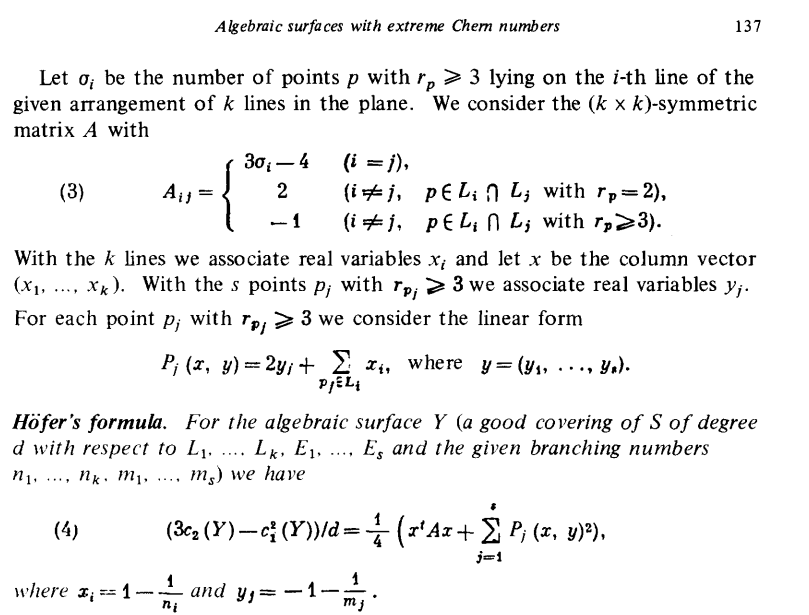
\includegraphics[width=0.8\textwidth,height=0.8\textheight,keepaspectratio]{hofer}
		\end{figure}
	\end{center}
\end{frame}


\begin{frame}
	\frametitle{The matroid polytope}
	\(\mH\) is an \emph{essential} and \emph{irreducible} hyperplane arrangement in \(\CP^n\)
	\vfill
	\begin{itemize}	
		\item A \textbf{basis} of \(\mH = \{H_1, \ldots, H_N\}\) is a subset \(\mB \subset \mH\) consisting of \(n+1\) linearly independent hyperplanes
		\vfill
		\item The indicator vector of \(\mB\) is the 1/0 vector
		\[
		\be_{\mB} = \sum_{i \,|\, H_i \in \mB} \be_i
		\]
		where \(\be_1, \ldots, \be_N\) are the standard basis vectors of \(\R^N\)
		\vfill
		\item The \textbf{matroid polytope} is the convex hull of the vectors \(\be_{\mB}\)
		\[
		P = \mathrm{conv} \{\, \be_{\mB} \,\,|\,\, \mB \, \text{ is a basis of } \mH \,\} 
		\]
	\end{itemize}
	Note: \(P\) is contained in the \((N-1)\)-simplex \(\Delta \subset \R^N\) with
	\[
	\Delta = \big\{\, (a_1, \ldots, a_N) \in \R^N \,|\, a_i \geq 0, \,\, \sum_i a_i = n+1 \, \big\}
	\]
\end{frame}


\begin{frame}
	\frametitle{The semistable and stable cones}
	\begin{itemize}
		\item The \textbf{semistable cone} is the cone over the matroid polytope
		\[
		C = \R_{\geq 0} \cdot P = \mathrm{cone} \,\, \{\, \be_{\mB} \,\,|\,\, \mB \, \text{ is a basis of } \mH \,\} 
		\]
		It is a convex polyhedral cone contained in the octant \(\big(\R_{\geq 0}\big)^N\)
		\vfill
		
		\item The \textbf{stable cone} is the interior of \(C \subset \R^N\)
		\[
		C^{\circ} = \mathrm{int} (C) 
		\]
		\vfill
		
		\item \(\mH\) is essential and irreducible \(\iff\) \(\dim P = N-1\)
		
		\phantom{\(\mH\) is essential and irreducible} \(\iff\) \(C^{\circ}\) is non empty
	\end{itemize}
\end{frame}


\begin{frame}
	\frametitle{Defining linear inequalities of the stable cone}
	\begin{itemize}
		\item Let \(\mL\) be the finite set of \emph{non-empty} and \emph{proper} linear subspaces \(L \subset \CP^n\) obtained by intersecting members of \(\mH\)
		
		\item \((a_1, \ldots, a_N) \in C^{\circ}\) \(\iff\) \(\forall i:\) \(a_i > 0\)  and \(\forall L \in \mL:\)
		\[
		\mathcolorbox{green!20}{
			\sum_{i \,|\, L \subset H_i} a_i < \frac{\codim L}{n+1} \cdot \sum_{i=1}^{N} a_i 
		}
		\]
	\end{itemize}

Relation to Geometric Invariant Theory:

\begin{itemize}
	\item Standard embedding \(\CP^n \subset \mathfrak{su}(n+1)^*\) as a coadjoint orbit
	
	Let \(p_i \in (\CP^n)^*\) be the annihilator of \(H_i\)
	
	\item \((a_1, \ldots, a_N) \in C^{\circ}\) \(\iff\) \(\exists\) \(F \in SL(n+1, \C)\) such that the centre of mass of the points \(F(p_i)\) with weights \(a_i\) is \(0 \in \mathfrak{su}(n+1)^*\)
	
	\item If \(n=1\) then \(\CP^1 = S^2\) and \(\mathfrak{su}(2)^* = \R^3\)
\end{itemize}
\end{frame}


\begin{frame}
	\frametitle{Main Result}
	\begin{theorem}[Miyaoka-Yau inequality, dB-Panov 2024]
		The Hirzebruch quadratic form is non-positive on the semistable cone:
		\[
		C \subset \{Q \leq 0\}
		\]
	\end{theorem}

\begin{itemize}
	\item If \(n=1\) then \(Q \equiv 0\)
	\item If \(n=2\) this follows from Panov's \emph{Polyhedral K\"ahler Manifolds}, Geometry \(\&\) Topology, 2009
	\item \textbf{Conjecture:} if \(\ba = (a_1, \ldots, a_N) \in C^{\circ}\) is such that \(Q(\ba) = 0\) and  \(a_i \in (0,1)\). Then there is a K\"ahler metric on \(\CP^n\) of constant holomorphic sectional curvature with cone angles \(2\pi\alpha_i\) in transverse directions to the hyperplanes \(H_i \in \mH\), with \(\alpha_i = 1-a_i\)
	\begin{itemize}
		\item If \(\mH\) is a complex reflection arrangement then the metrics have been constructed by Couwenberg-Heckman-Looijenga (IH\'ES, 2005)
	\end{itemize}
\end{itemize}
\end{frame}


\begin{frame}
	\frametitle{klt and CY arrangements}
	A weighted arrangement is a pair \((\mH, \ba)\) consisting of:
	\begin{itemize}
		\item a hyperplane arrangement \(\mH\) in \(\CP^n\)
		\item a weight vector \(\ba \in \R^{\mH}\) with components \(a_H > 0\)
	\end{itemize}
	
	
	
	
	The weighted arrangement \((\mH, \ba)\) is
	\begin{itemize}
		\item  klt if
		\[
		\mathcolorbox{yellow!20}{
	\forall L \in \mL: \,\, \sum_{H \supset L} a_H < \codim L 	
	}
		\] 
		where \(\mL\) is the set of non-empty and proper subspaces \(L \subset \CP^n\) obtained by intersecting hyperplanes in \(\mH\).
		In particular, 
		\[0 < a_H < 1 \]
		\item  Calabi-Yau (CY) if
		\[
		\mathcolorbox{yellow!20}{
			\sum_{H \in \mH} a_H = n+1 	
		}
		\] 
	\end{itemize}
\end{frame}


\begin{frame}
	\frametitle{Restatement of the main theorem}
	\begin{theorem}[Miyaoka-Yau inequality, dB-Panov 2024]
		Suppose that the weighted arrangement \((\mH, \ba)\) is klt and CY. Then
		\[
		Q(\ba) = \sum_{L \in \mLi^{n-2}} a_L^2 \,-\, \frac{1}{2} \sum_{H \in \mH} B_H \cdot a_H^2 \,-\, \frac{n+1}{2} \leq 0 
		\]
	\end{theorem}
\begin{itemize}
	\item \(\mLi^{n-2}\) is the set of irreducible codimension \(2\) subspaces \(L \subset \CP^n\)
	\item The weight \(a_L\) at \(L \in \mLi^{n-2}\) is given by
	\[
	a_L = \frac{1}{2} \cdot \sum_{H \supset L} a_H
	\]
	\item \(B_H + 1\) is the number of \(L \in \mLi^{n-2}\) with \(L \subset H\)
\end{itemize}
\end{frame}


\begin{frame}
	\frametitle{Sketch proof: the resolution}
	\begin{itemize}
		\item Logarithmic resolution
		\[
		X \xrightarrow{\pi} \CP^n
		\]
		with \(D = \pi^{-1}(\mH)\) a simple normal crossing divisor
		
		\item \(X\) is the \emph{minimal De Concini-Procesi wonderful model} of \(\mH\)
		
		\item The irreducible components of \(D\) are in bijective correspondence with non-empty and proper irreducible subspaces \(L \in \mLi\) 
		\[
		D = \bigcup_{L \in \mLi} D_L
		\]
		where \(D_L\) is the unique irreducible component of \(D\) such that 
		\[
		\pi(D_L) = L 
		\]
		
	\end{itemize}
\end{frame}

\begin{frame}
	\frametitle{Sketch proof: the resolution (example)}
	Let \(p_1, \ldots, p_5 \in \CP^3\) be five points in general linear position
	
	\vspace{-1mm}
	\begin{center}
		\(\mH \,\,=\,\, \)\(10\) planes \(\overline{p_i p_j p_k}\)
	\end{center}
	\vspace{-1mm}
	
	\begin{columns}
		\begin{column}{.3\textwidth}
		\begin{figure}[H]
			\centering
			\scalebox{.6}{
			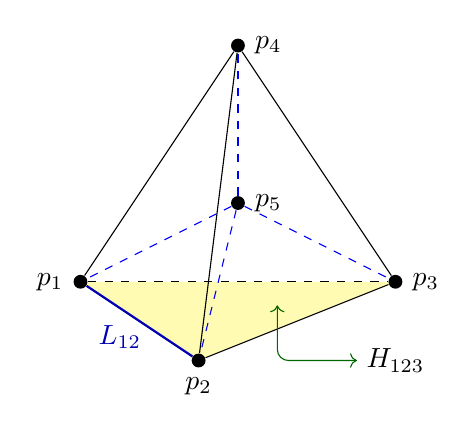
\begin{tikzpicture}
				
				\fill[yellow!30] (0,0) -- (4,0) -- (1.5,-1);
				
				\node[circle,fill=black,inner sep=0pt,minimum size=5pt,label=left:{$p_1$}] (x1) at (0,0) {};
				\node[circle,fill=black,inner sep=0pt,minimum size=5pt,label=right:{$p_3$}] (x3) at (4,0) {};
				\node[circle,fill=black,inner sep=0pt,minimum size=5pt,label=right:{$p_4$}] (x4) at (2,3) {};
				\node[circle,fill=black,inner sep=0pt,minimum size=5pt,label=below:{$p_2$}] (x2) at (1.5,-1) {};
				\node[circle,fill=black,inner sep=0pt,minimum size=5pt,label=right:{$p_5$}] (x5) at (2,1) {};
				
				\draw (x1) -- (x2) -- (x3) -- (x4) -- (x1);
				\draw (x4) -- (x2);
				\draw[dashed] (x1) -- (x3);
				\draw[dashed, blue] (x5) -- (x1);
				\draw[dashed, blue] (x5) -- (x2);
				\draw[dashed, blue] (x5) -- (x3);
				\draw[dashed, blue] (x5) -- (x4);
				
				\node (h) at (4,-1) {\(H_{123}\)};
				\draw[<->, rounded corners, black!60!green] (2.5,-.3) -- (2.5, -1) -- (h);
				\node[black!30!blue] (l) at (.5,-.7) {\(L_{12}\)};
				\draw[thick, black!30!blue] (x1) -- (x2);
			\end{tikzpicture}
		}
			%\caption{The arrangement \(\mH\) of \(10\) planes in \(\CP^3\) spanned by triplets of \(5\) points in general linear position.}
			%\label{fig:tetra}
		\end{figure}	
		\end{column}
		\begin{column}{.68\textwidth}
			\begin{itemize}
				\item \textbf{Step 1:} \(X_1 \xrightarrow{\sigma_1} \CP^3\) is the blowup at the five points \(p_i\)
				
				\item \textbf{Step 2:} \(X \xrightarrow{\sigma_2} X_1\) is the blowup at the \(10\) (disjoint) proper transforms of the  lines \(L_{ij}\)
			\end{itemize}
		\end{column}
	\end{columns}
	
\footnotesize{
	\begin{equation*}	
		\pi^{-1}(\mH) = \underbrace{\left( \bigcup_{H} D_H \right)}_{10 \text{ divisors } \cong \Bl_4 \P^2} \bigcup \underbrace{\left( \bigcup_{L} D_L \right)}_{10 \text{ divisors } \cong \P^1 \times \P^1} \bigcup \underbrace{\left( \bigcup_{p} D_p \right)}_{5 \text{ divisors } \cong \Bl_4 \P^2} 
	\end{equation*}
}	
\vfill
\normalsize	
\textbf{Remark:} \(X = \overline{M_{0,6}}\)

\end{frame}

\begin{frame}
	\frametitle{Sketch proof: the parabolic bundle}
	Parabolic bundle \(\mE_{*}\) on \((X,D)\) defined by:
	\begin{itemize}
		\item vector bundle \(\mE = \pi^*(T\CP^n)\)
		\item weights \(a_L\) for \(L \in \mLi\) given by
		\[
		a_L = (\codim L)^{-1} \sum_{H \supset L} a_H 
		\]
		\item increasing filtrations of \(\mE|_{D_L}\) by vector subbundles 
		\begin{equation*}
		F^L_a = 
		\begin{cases}
		\pi^*(TL) &\text{ if } a < a_L \\
		\mE|_{D_L} &\text{ if } a \geq a_L 
		\end{cases}
		\end{equation*}	
	\end{itemize}
\emph{Remark:} klt implies \(a_L \in (0,1)\) and 
CY implies \(\mathcolorbox{yellow!20}{\parc_1(\mE_{*}) = 0}\)
\end{frame}


\begin{frame}
	\frametitle{Sketch proof: the stability theorem}
	\begin{itemize}
		\item Fix positive integers \(b_L\) for \(L\) in \( \mLi^{\circ} = \mLi \setminus \mH\) such  that
		\begin{equation*}
		P_k = k \cdot \pi^*\big(\mO_{\P^n}(1)\big) - \sum_{L \in \mLi^{\circ}} b_L \cdot D_L
		\end{equation*}
		is an ample line bundle on \(X\) for all \(k \gg 1\)
		\vfill
		
		\item \textbf{Stability Theorem.}
		If \(\mV \subset \mE\) is a non-zero and proper \emph{saturated subsheaf}. Then
		\[
		\parc_{1}(\mV_{*}) \cdot c_1(P_k)^{n-1} < 0 
		\]
		where \(\mV_{*}\) is the naturally induced parabolic structure on \(\mV\)
	\end{itemize}
\end{frame}


\begin{frame}
	\frametitle{Sketch proof: the Bogomolov-Gieseker inequality}
	\begin{itemize}
		\item The Bogomolov-Gieseker inequality for stable parabolic bundles (proved by Takuro Mochizuki in 2006, \emph{Ast\'erisque}) asserts that
		\[
	   \parch_2(\mE_{*}) \cdot 	c_1(P_k)^{n-2}  \leq 0 
		\]
		\vfill
		\item The expression \(\parch_2(\mE_{*}) \cdot 	c_1(P_k)^{n-2}\) defines a polynomial of degree \(n-2\) in \(k\) that we write as \(p(k)\)
		\vfill
		\item Calculation of \(\parch_2(\mE_{*})\) and certain cup products in \(H^*(X)\) show that
		\[
		p(k) = Q(\ba) \cdot k^{n-2} + O(k^{n-3}) 
		\]
		\vfill
		\item Since \(p(k)<0\) for \(k \gg 1\)\,, we must have \(Q(\ba) \leq 0\) \hspace{3mm}  \(\square\)
	\end{itemize}
\end{frame}


\begin{frame}
	\frametitle{Stability Theorem and distributions on \(\CP^n\)}
	\begin{block}{Key estimate}
		Suppose that \((\mH, \ba)\) is a weighted arrangement that is  klt and CY.
		Then there is \(\delta>0\) such that, for any distribution \(\mV \subset T\CP^n\) with index \(\imath = c_1(\mV) \geq 0\), we have
		\begin{equation*}
		\sum_{H  | H \pitchfork \mV} a_H \geq \imath + \delta  \,,
		\end{equation*}
		where the sum is over all \(H \in \mH\) that are transverse to \(\mV\).
	\end{block}

\textbf{Example.}
Let \(M \subset \CP^n\) be a linear subspace with \(\dim M = r-1\) for some \(1 \leq r \leq n-1\). The collection of all \(r\)-dimensional subspaces that contain \(M\) defines a distribution \(\mV \cong \mO_{\P^n}(1)^{\oplus r}\) of index \(\imath = r\). 

A hyperplane is tangent to \(\mV\) if and only if \(H \supset M\). 
\end{frame}

\begin{frame}
	\frametitle{Application: lower bound on total sum of multiplicities}
	%\(\mH = \{H_1, \ldots, H_N\}\) and \(t_i =\) number of \(L \in \mL^{n-2}\) with \(L \subset H_i\)
	\begin{theorem}[dB-Panov, 2024]\label{thm:hir}
		Suppose that for all \(L \in \mL\) we have
		\begin{equation*}
		m_L < \codim L \cdot \frac{N}{n+1} \hspace{3mm} \big(\,i.e.\,\, \mathbf{1} \in C^{\circ} \,\big)
		\end{equation*}
		Then
		\begin{equation*}
		\sum_{L \in \mL^{n-2}} m_L \geq \left( 1 - \frac{2}{n+1} \right) N^2 + N \hspace{3mm} \big(\,i.e.\,\, Q(\mathbf{1}) \leq 0 \,\big)
		\end{equation*}
		Equality holds if and only if every \(H \in \mH\) intersects \(\mH \setminus \{H\}\) along
		\begin{equation*}
		\left( 1 - \frac{2}{n+1} \right) N + 1 \hspace{3mm} \big(\,i.e.\,\, \mathbf{1} \in \ker Q \,\big)	
		\end{equation*}
		codimension \(2\) subspaces.
	\end{theorem}
\end{frame}
%The set of all hyperplanes of a finite projective space satisfies \eqref{eq:sthir} bit does not satisfy \eqref{eq:hirineq}


\begin{frame}
	\frametitle{Hirzebruch arrangements}
	A hyperplane arrangement \(\mH\) is Hirzebruch if:
	\begin{itemize}
		\item for every subspace \(L \in \mL\) we have
		\begin{equation*}
		\mathcolorbox{green!20}{
		\frac{m_L}{\codim L} \leq \frac{N}{n+1}
		} 
		\end{equation*}
		
		\item every \(H \in \mH\) intersects the others along
		\begin{equation*}
		\mathcolorbox{green!20}{
		\left( 1 - \frac{2}{n+1} \right) N + 1
		} 
		\end{equation*}
		codimension \(2\) subspaces.
	\end{itemize}

\textbf{Examples:} (i) The \(n+1\) coordinate hyperplanes in \(\CP^n\).

(ii) If \(\mH \subset \CP^1\) and \(|\mH| \geq 2\) then \(\mH\) is Hirzebruch. 

However, if \(n\geq 2\) then the Hirzebruch condition is more rigid.

\end{frame}

\begin{frame}
	\frametitle{Complex reflection groups}
	\begin{itemize}
		\item \(G \subset U(n+1)\) irreducible complex reflection group
		\item \(\mH = \) reflecting hyperplanes
	\end{itemize}

	\begin{theorem}[dB-Panov, 2024]
		\(\mH\) is Hirzebruch and its quadratic form \(Q\) is negative semidefinite
	\end{theorem}
	
	\emph{Proof:} show that \(\mathbf{1} \in C^{\circ}\) and \(Q(\mathbf{1}) = 0\). Key identity:
	\[
	\sum_{H \in \mH} | \langle v, n_H \rangle |^2 = \frac{N}{n+1} \cdot \| v \|^2  
	\]
	which follows from Schur's lemma. \,\, \(\square\)
	
	\textbf{Example:} Take in $\mathbb CP^{n+1}$ the plane $\mathbb CP^n=\{x_1+\ldots+x_{n+2}=0\}$.
	
	The \emph{braid arrangement} $A_{n+1}\subset\mathbb CP^n$ is given by planes $x_i-x_j=0$ for $i\ne j\in \{1,\ldots,n+2\}$.
	$A_{n+1}$ consists of $(n+1)(n+2)/2$ hyperplanes and induces $A_n$ on each of them.
\end{frame}


\begin{frame}
	\frametitle{Hirzebruch line arrangements/Geometrization}
	
	{\bf Hirzebruch's problem 1985.} Consider an arrangement of \(N\) lines in $\mathbb CP^2$ such that each line intersects others in exactly \(N/3 + 1\) points. Does such an arrangement consist of mirrors of a finite reflection group?
	
	\vspace{-1mm}
	\begin{figure}[!h]
		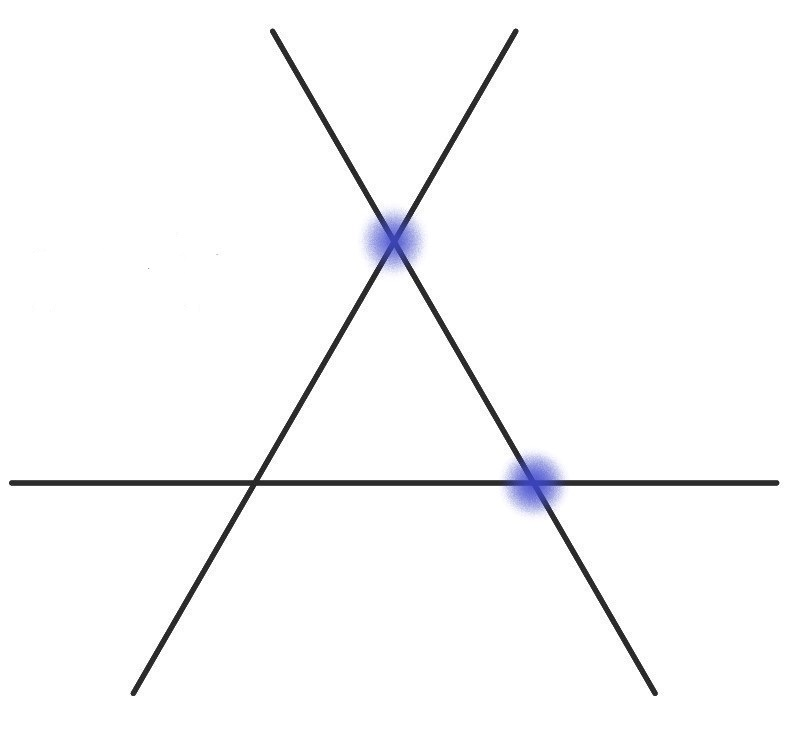
\includegraphics[scale=.1]{Hirzebruch1}
		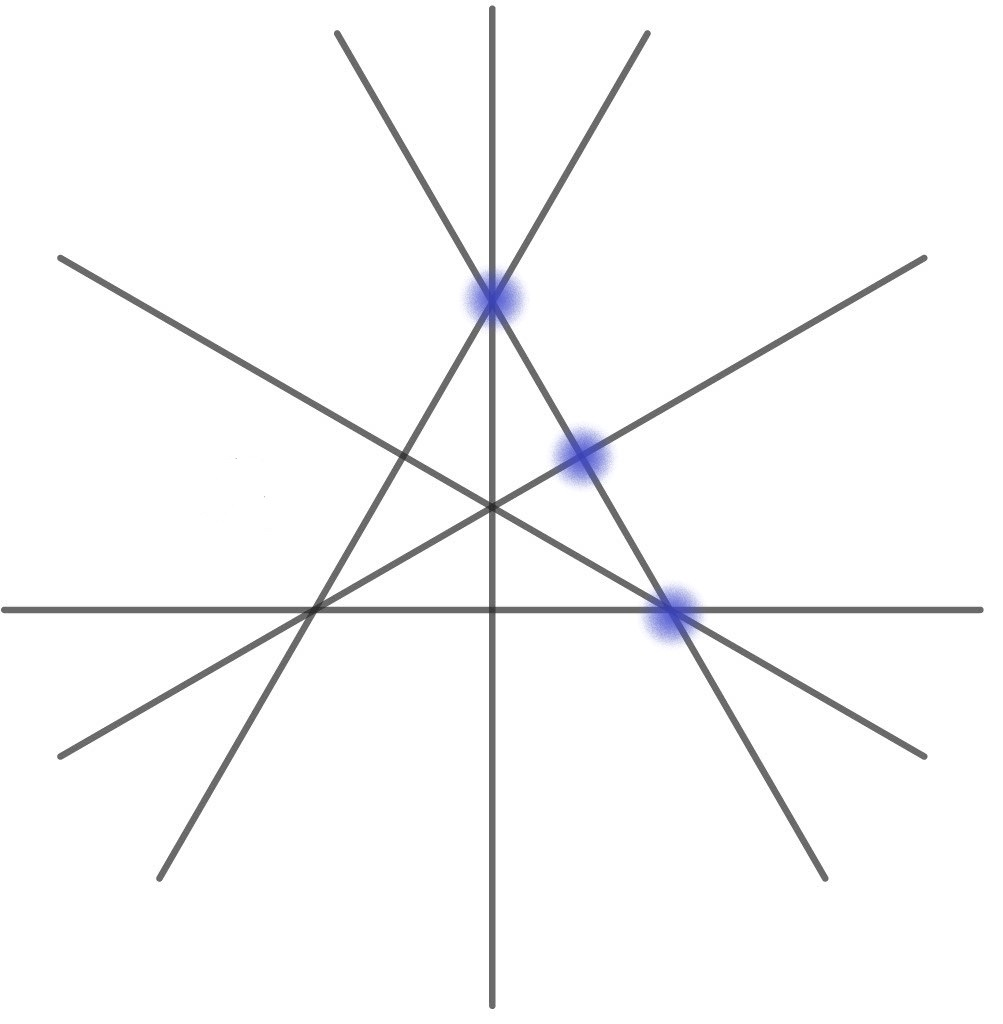
\includegraphics[scale=.1]{Hirzebruch2}
		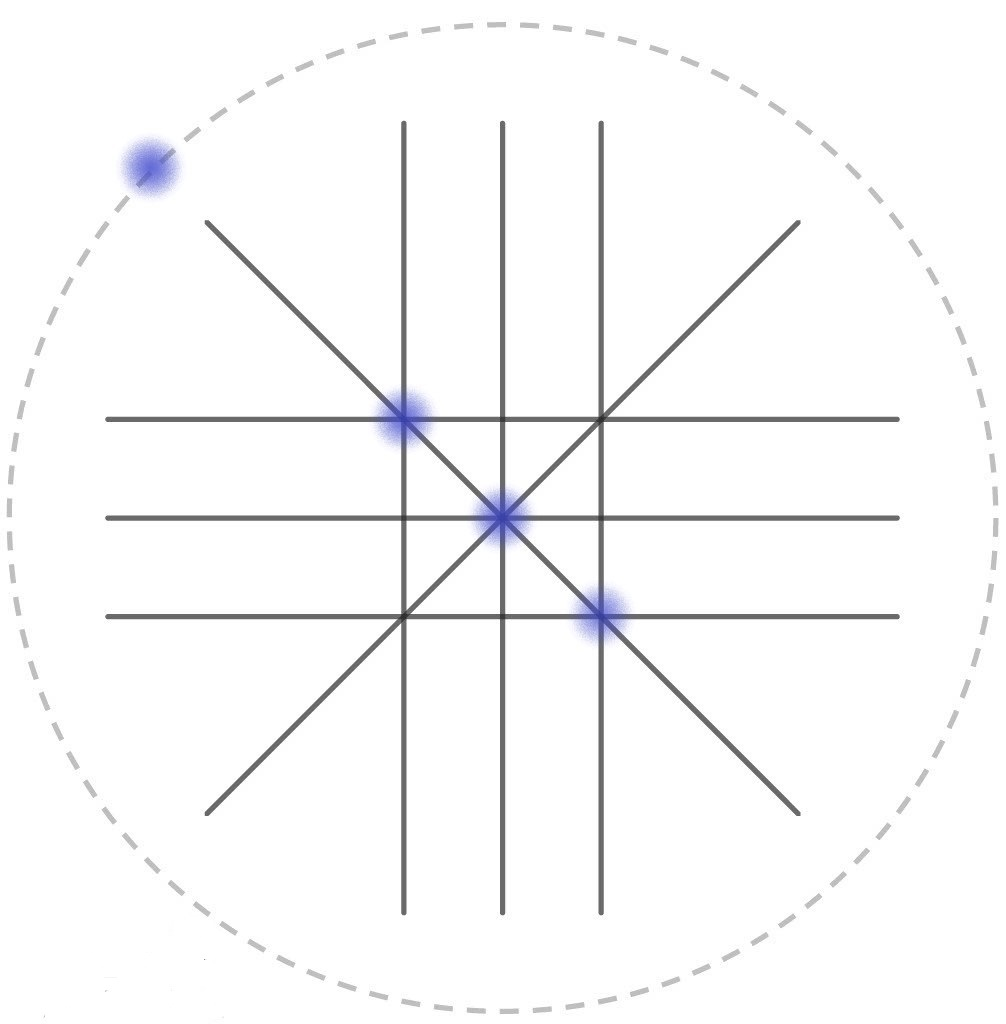
\includegraphics[scale=.1]{Hirzebruch3}
		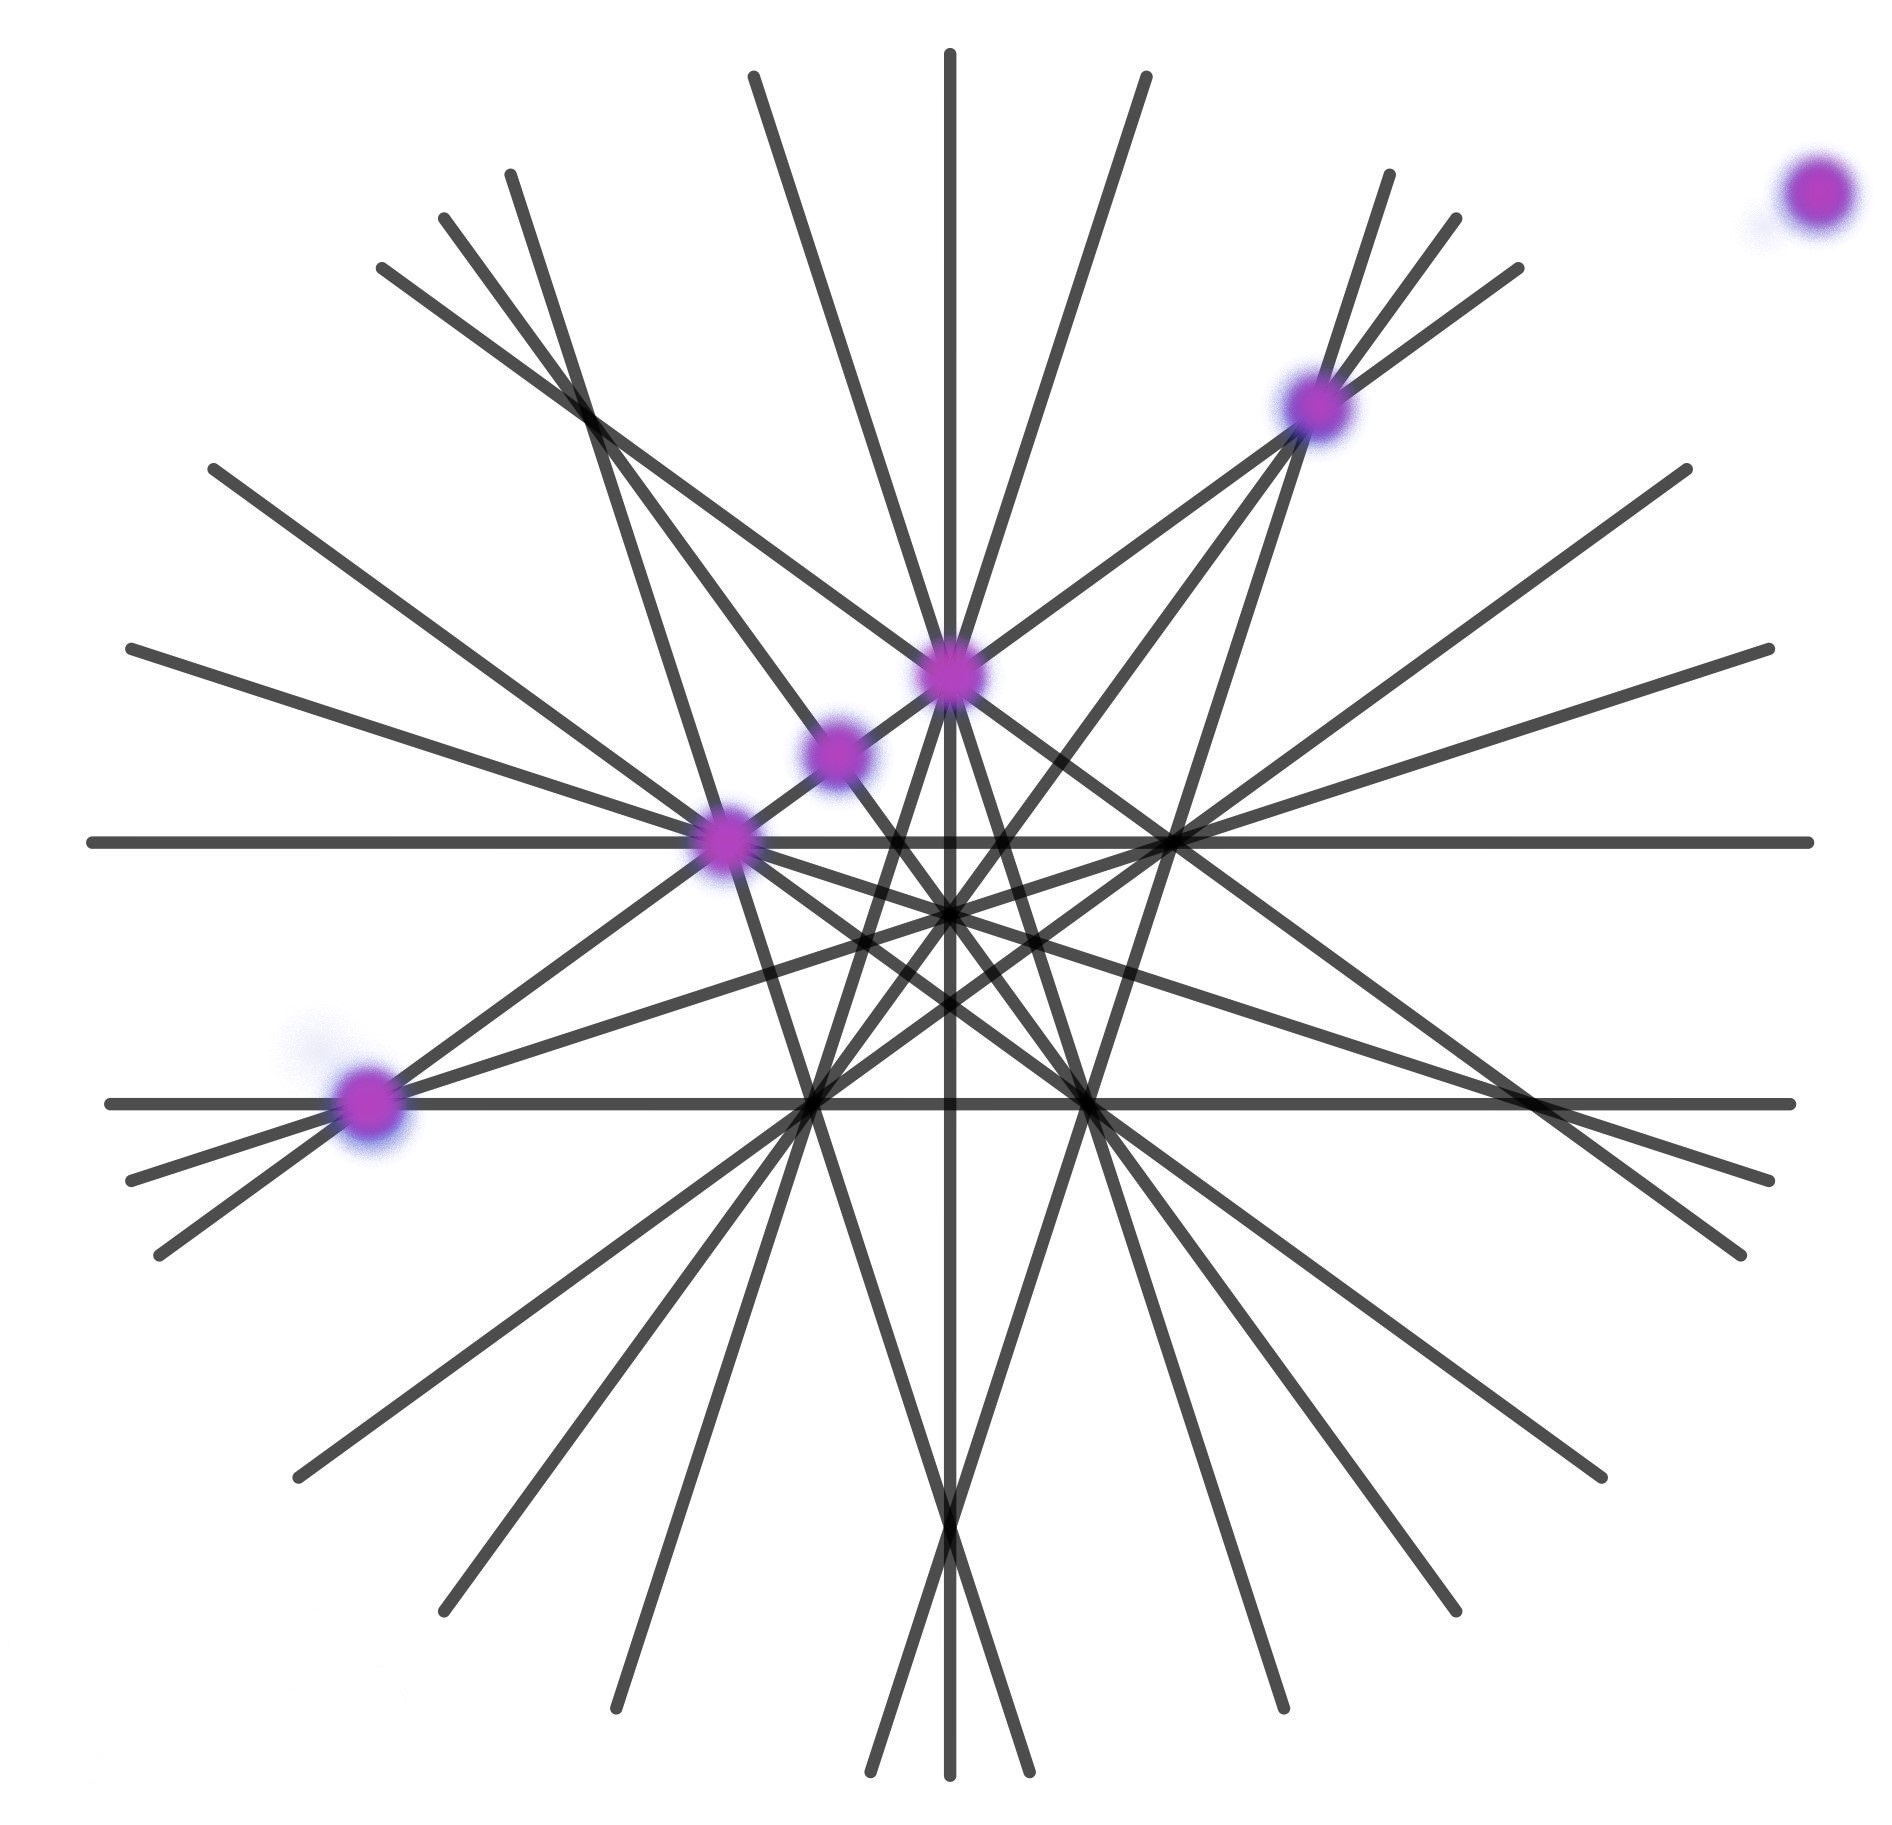
\includegraphics[scale=.05]{Hirzebruch5}
	\end{figure}
	
	\vspace{-1mm}
	\begin{figure}[!h]
		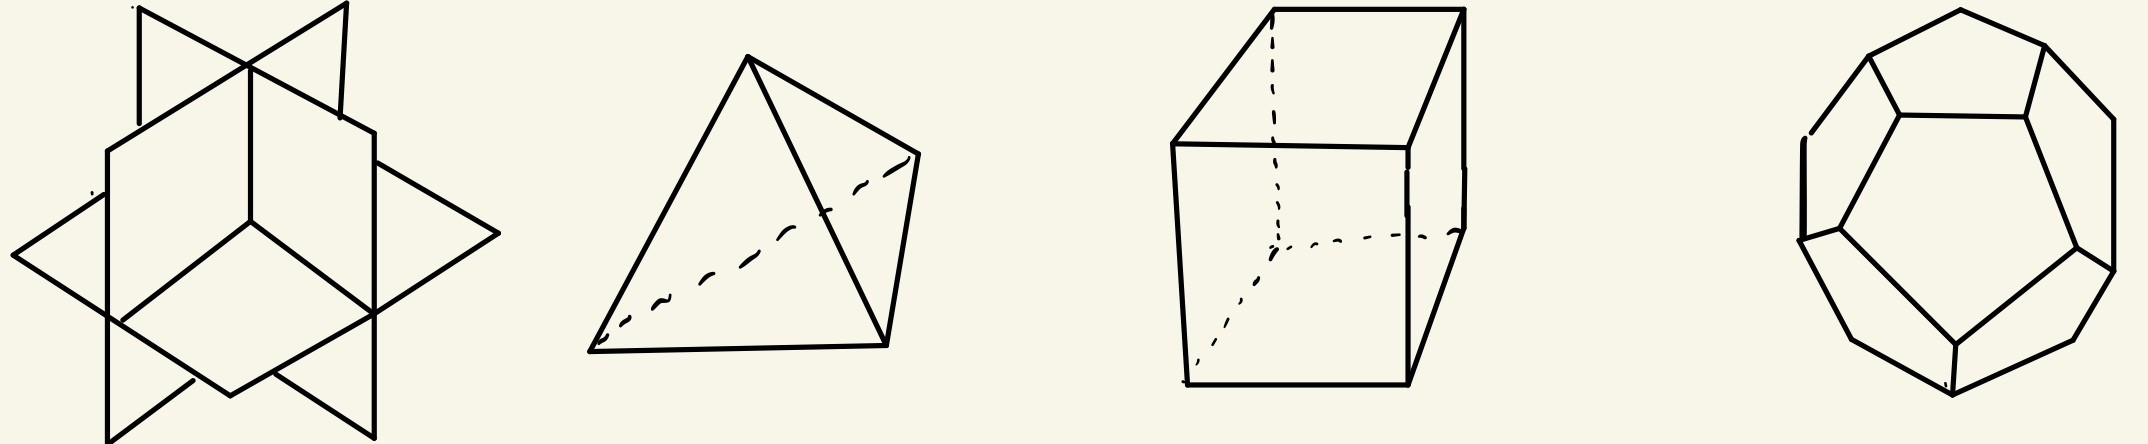
\includegraphics[scale=.15]{platon}
	\end{figure}
	
	Panov (Geometry \& Topology, 2018): there exist exactly four Hirzebruch line arrangements in \(\mathbb{RP}^2\)
\end{frame}

\begin{frame}
	\frametitle{Example: Non-Pappus matroid}
	
	\begin{columns}
		\begin{column}{.4\textwidth}
		\begin{figure}[h]
			\centering
			\scalebox{.5}{
				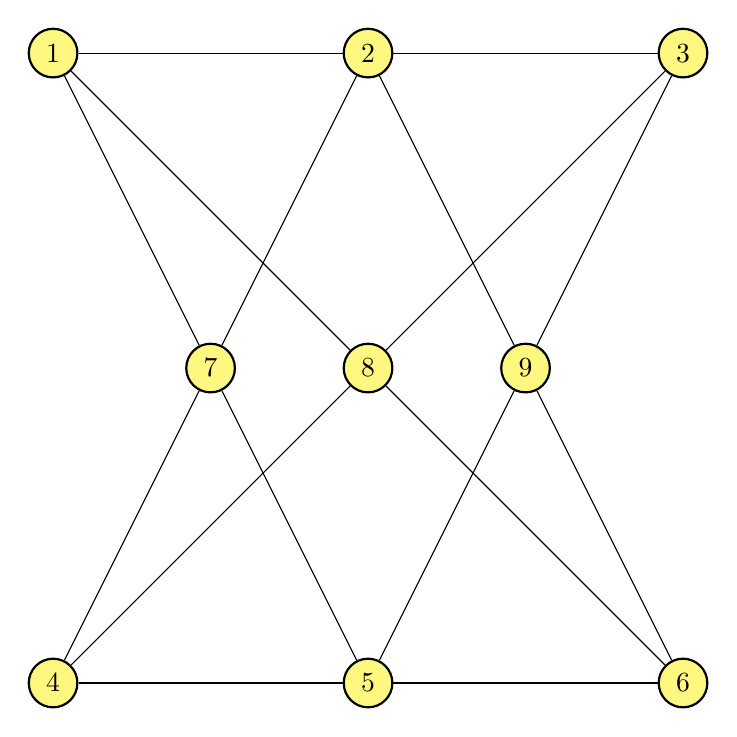
\begin{tikzpicture}
					\node (1) at (-4,4) [thick,circle,draw,fill=yellow!50] {\(1\)};
					\node (2) at (0,4) [thick,circle,draw,fill=yellow!50] {\(2\)};
					\node (3) at (4,4) [thick,circle,draw,fill=yellow!50] {\(3\)};
					\node (7) at (-2,0) [thick,circle,draw,fill=yellow!50] {\(7\)};
					\node (8) at (0,0) [thick,circle,draw,fill=yellow!50] {\(8\)};
					\node (9) at (2,0) [thick,circle,draw,fill=yellow!50] {\(9\)};
					\node (4) at (-4,-4) [thick,circle,draw,fill=yellow!50] {\(4\)};
					\node (5) at (0,-4) [thick,circle,draw,fill=yellow!50] {\(5\)};
					\node (6) at (4,-4) [thick,circle,draw,fill=yellow!50] {\(6\)};
					
					\draw (1) -- (2) -- (3);
					\draw (4) -- (5) -- (6);
					
					\draw (1) -- (7) -- (5);
					\draw (2) -- (7) -- (4);
					
					\draw (2) -- (9) -- (6);
					\draw (3) -- (9) -- (5);
					
					\draw (1) -- (8) -- (6);
					\draw (3) -- (8) -- (4);
				\end{tikzpicture}
			}
			%\caption{The Non-Pappus matroid.}
			\label{fig:nonpapus}
		\end{figure}	
		\end{column}
		
		\begin{column}{.68\textwidth}
			\small{
			\[
			\begin{pmatrix}
				-5 & 1 & 1 & -2 & 1 & 1 & 1 & 1 & -2 \\
				1 & -5 & 1 & 1 & -2 & 1 & 1 & -2 & 1 \\
				1 & 1 & -5 & 1 & 1 & -2 & -2 & 1 & 1 \\
				-2 & 1 & 1 & -5 & 1 & 1 & 1 & 1 & -2 \\
				1 & -2 & 1 & 1 & -5 & 1 & 1 & -2 & 1 \\
				1 & 1 & -2 & 1 & 1 & -5 & -2 & 1 & 1 \\
				1 & 1 & -2 & 1 & 1 & -2 & -2 & -2 & -2 \\
				1 & -2 & 1 & 1 & -2 & 1 & -2 & -2 & -2 \\
				-2 & 1 & 1 & -2 & 1 & 1 & -2 & -2 & -2
			\end{pmatrix}
			\, 
			\]
		}
		\end{column}
	\end{columns}
		
	The Hirzebruch quadratic form is \(\leq 0\) on the positive octant of \(\R^9\).
	\vfill
	
	\textbf{Question:} does Miyaoka-Yau inequality holds for oriented matroids?
	\vfill
	\textbf{Open problem:} do symplectic \(4\)-manifolds of `general type' satisfy \(c_1^2 \leq 3c_2\) ?
	
	\begin{center}
		THANK YOU!
	\end{center}
\end{frame}



\end{document}


